
% This LaTeX was auto-generated from an M-file by MATLAB.
% To make changes, update the M-file and republish this document.

\documentclass{article}
\usepackage{graphicx}
\usepackage{color}

\sloppy
\definecolor{lightgray}{gray}{0.5}
\setlength{\parindent}{0pt}

\begin{document}

    
    
\section*{Lorenz Attractor}

\begin{par}
The Lorenz system is a well known example of deterministic chaos in a simple set of 3 ordinary differential equations. This example illustrates the use of 3D visualization in understanding the phase plane dynamics of a simple nonlinear system.
\end{par} 
\begin{par}
$$ \frac{dx}{dt} = \sigma(y - x) $$
$$ \frac{dy}{dt} = $$
$$ \frac{dz}{dt} = $$
\end{par} \vspace{1em}

\subsection*{Contents}

\begin{itemize}
\setlength{\itemsep}{-1ex}
   \item Dependencies
   \item Parameters
   \item Model Equations
   \item Simulation
   \item Lorenz Attractor
\end{itemize}


\subsection*{Dependencies}

\begin{par}
This example uses the Chebfun package.
\end{par} \vspace{1em}


\subsection*{Parameters}

\begin{verbatim}
sig=10;
beta=8/3;
rho=28;
\end{verbatim}


\subsection*{Model Equations}

\begin{verbatim}
deriv = @(t,x) [ ...
    -sig*x(1) + sig*x(2); ...
    rho*x(1) - x(2) - x(1)*x(3); ...
    -beta*x(3) + x(1)*x(2)];
\end{verbatim}


\subsection*{Simulation}

\begin{verbatim}
y = ode45(deriv,domain(0,80),[3 0 5]);

figure(1);clf;
subplot(3,1,1); plot(y(:,1)); ylabel('y_1');
title('Lorenz Oscillator');
subplot(3,1,2); plot(y(:,2)); ylabel('y_2');
subplot(3,1,3); plot(y(:,3)); ylabel('y_3');
xlabel('Time');
\end{verbatim}

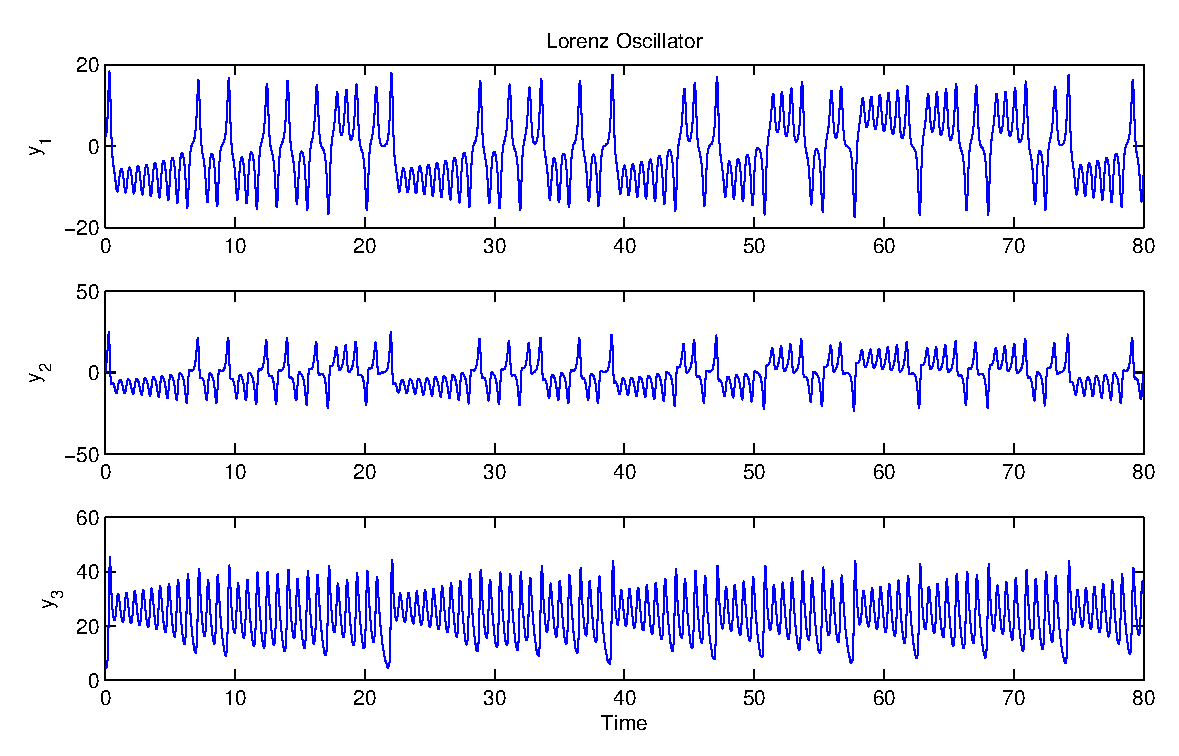
\includegraphics [width=4in]{Ch02_Lorenz_chebfun_01.eps}


\subsection*{Lorenz Attractor}

\begin{verbatim}
figure(2);clf;
plot3(y(:,1),y(:,2),y(:,3));
grid
title('Lorenz Oscillator');
xlabel('y_1');ylabel('y_2');zlabel('y_3');
\end{verbatim}

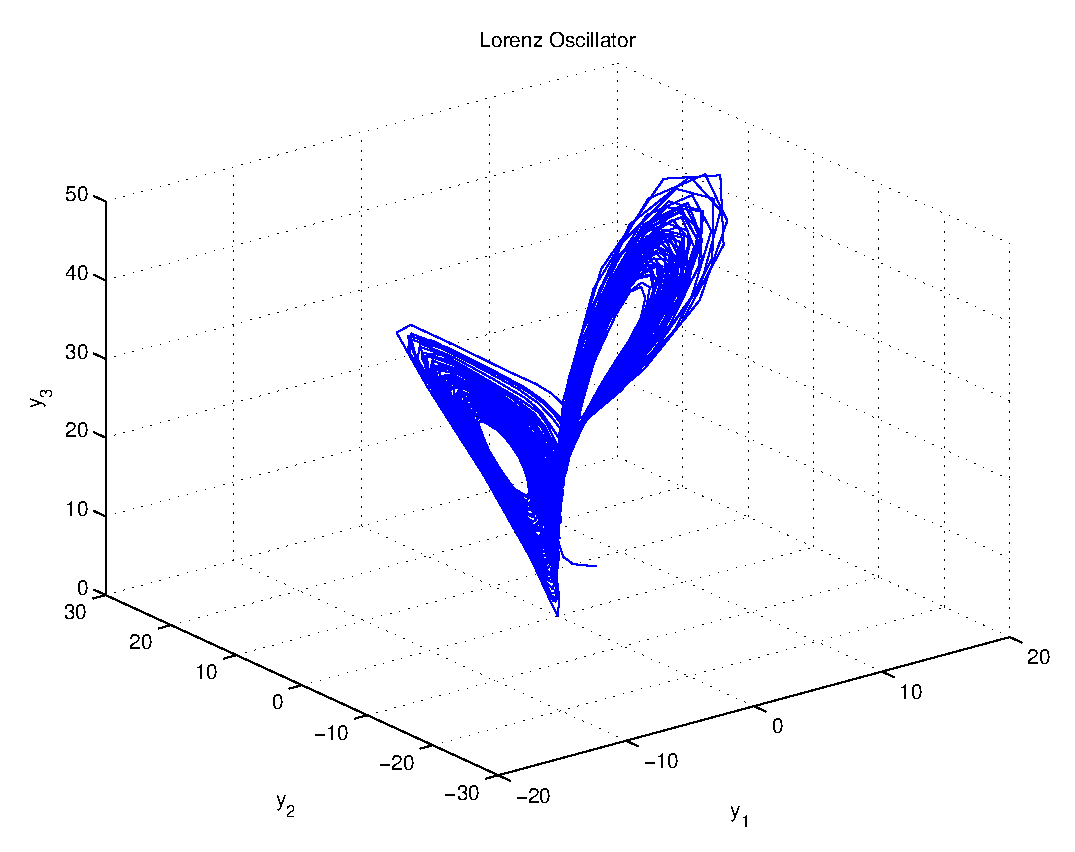
\includegraphics [width=4in]{Ch02_Lorenz_chebfun_02.eps}



\end{document}
    
